\documentclass{article}
\usepackage[parfill]{parskip}
\usepackage[a4paper, total={6in, 9in}]{geometry}

\usepackage{titlesec}
\titlespacing*{\section}{0pt}{0.01\baselineskip}{0.01\baselineskip}

\usepackage{graphicx} %Paquete para incluir imagenes

\titleformat{\paragraph}
{\normalfont\normalsize\bfseries}{\theparagraph}{1em}{}
\titlespacing*{\paragraph}
{0pt}{3.25ex plus 1ex minus .2ex}{1.5ex plus .2ex}


\graphicspath{ {./images/} }
%\usepackage[margin=1cm]{geometry} % Centra el texto

\begin{document}

\begin{titlepage}
  \vspace*{1cm}

  \begin{center}
    {\Huge{Informe del Trabajo Practico 1}}
  \end{center}

  \vspace{0.4cm}

  \begin{center}
    {\LARGE{Facultad de Ingeniería de la Universidad de Buenos Aires}}\\
    \vspace{0.3cm}
  \end{center}

  \vspace{0.8cm}
  \begin{center}
    
\includegraphics[scale=0.8]{Logo-fiuba}
  \end{center}

  \vspace{0.4cm}
  \begin{center}
    {\Large{Grupo 09}}\\
    \vspace{0.6cm}
    {\begin{minipage}[t]{.32\textwidth}
        \begin{center}
	Castro  Martinez, Jose Ignacio\\
          {\small{Padrón: 106957}}\\
          {\small{email: jacastrom@fi.uba.ar}}
        \end{center}
	\end{minipage}
	\begin{minipage}[t]{.32\textwidth}
        \begin{center}
	Douce, German Alejandro\\
          {\small{Padrón: 106001}}\\
          {\small{email: gdouce@fi.uba.ar}}\\
        \end{center}
      \end{minipage}
      \begin{minipage}[t]{.32\textwidth}
        \begin{center}
          Orsi, Tomas Fabrizio\\
          {\small{Padrón: 109735}}\\
          {\small{email: torsi@fi.uba.ar}}
        \end{center}
      \end{minipage}}
  \end{center}
\end{titlepage}

\section*{Hotels}
El data frame está compuesto por un conjunto de 61913 filas (registros) y 31 columnas en donde cada registro representa una reserva de hotel y cada columna es una variable distinta que brinda información acerca de dichas reservas. El objetivo de esta primera parte es realizar un análisis exploratorio del DataFrame e identificar Outliers para poder trabajar con uno más “limpio” a la hora de predecir nuestra variable target: “is\_cancelled”. Variables con pocos valores que tienen mucha desviación podrían generar “ruido” y falsas tendencias en las reservas a cancelar por sí o por no. También se puede hacer una predicción más “honesta” evitando sesgos sobre algunas variables.
El notebook se divide de la siguiente manera:

\begin{itemize}
	\item Preparación del ambiente de trabajo
	\item Análisis univariado
	\begin{itemize}
		\item Cuantitativas
		\item Cualitativas
	\end{itemize}
	\item Análisis multivariado
	\item Relación contra el target: “is\_canceled”
\end{itemize}
\subsection*{Preparación del ambiente de trabajo}
En esta sección, realizamos los imports necesarios para trabajar con el Data Frame. Luego mostramos algunos registros y listamos las columnas con sus tipos de datos. Además, cambiamos los nombres de las variables por otros más declarativos.

\subsection*{Análisis univariado}
Listamos las variables y las dividimos en Cualitativas y Cuantitativas. De las 31 variables, 16 son cuantitativas y 15 son cualitativas.
\subsection*{Cuantitativas}
Para cada una de ellas:
\begin{itemize}
	\item Vemos sus valores estadísticos más relevantes;
	\item Detectamos la cantidad de valores nulos;
	\item Construimos una gráfica de distribución de sus valores en algunos casos gráficas de tipo boxplot para identificar más fácilmente valores atípicos (Outliers) y en el caso de la variable “average\_daily\_rate” agregamos un análisis con Z\_score;
	\item Realizamos un tratamiento sobre dichos valores eliminando sus registros o reemplazando los valores atípicos por otros.
\end{itemize} 
Para estas variables concluimos lo siguiente:
\begin{itemize}
	\item La única variable con datos nulos o faltantes es “babies\_number”;
	\item  Decidimos eliminar la variable “previous booking not cancelled” debido a que, después de remover unos pocos valores outliers, todo el resto de los registros presentan el mismo valor. Esto no nos aporta ningún tipo de información
\end{itemize}

\subsection*{Cualitativas}
Para estas, en primer lugar analizamos las variables con valores nulos. Estas fueron: “agent\_id”, “company\_id” y “country” de las cuales se decidió eliminar company\_id  por contener un 92\% de valores faltantes.\\
Para cada una de ellas:
\begin{itemize}
	\item Mostramos los valores que toman;
	\item Realizamos una gráfica de distribución de sus valores
	\item En el caso de “agent\_id” y “country” se corrigieron sus valores valores faltantes
\end{itemize}

\subsection*{Análisis multivariado}

En esta sesión hicimos multivariado entre las siguientes parejas de variables. En algunos de ellos encontramos algunos Outliers que luego eliminamos y en otros no. Además agregamos la columna “dias\_totales” al Data Frame.

\begin{itemize}
	\item “weekend nights” vs “weekend nights num” (de las suma de estas 2 nace la columna dias totales)
	\item adr vs customer Type
	\item room type vs adr
	\item Children Num vs Babies num vs Adult Num
\end{itemize}

\subsection*{Relación contra el target: “is\_canceled”}
Se realizaron gráficas de las siguientes variables comparándolas contra el target. 

\begin{itemize}
	\item Lead Time
	\item Previous\_cancellations\_num
	\item Average\_daily\_rate
	\item dias\_totales
	\item reserved\_room\_type
\end{itemize}

De las n variables analizadas la única que parecería tener cierta influencia directa en el target es “Lead time”. Su gráfica podría sugerir que reservas realizadas con mayor anticipación tendrían más probabilidad de ser canceladas. \\
El resto de las gráficas tienen distribuciones muy homogéneas al hacer foco en el número de reservas canceladas. Mostramos abajo a la derecha una distribución homogénea, y a la izquierda la distribución de Lead Time.

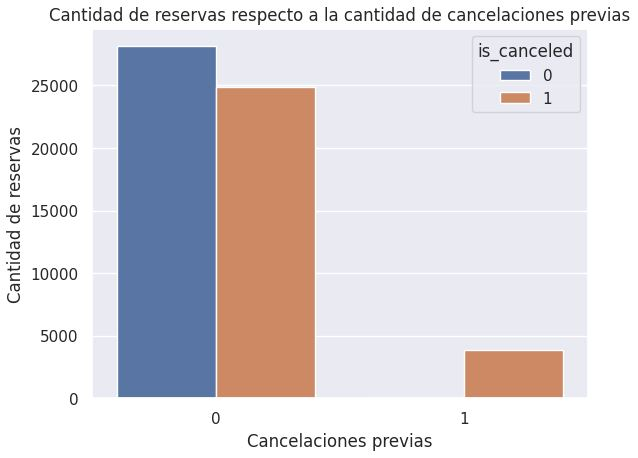
\includegraphics[scale=0.2]{previous_cancellations_num}
    \hspace{4.5cm}
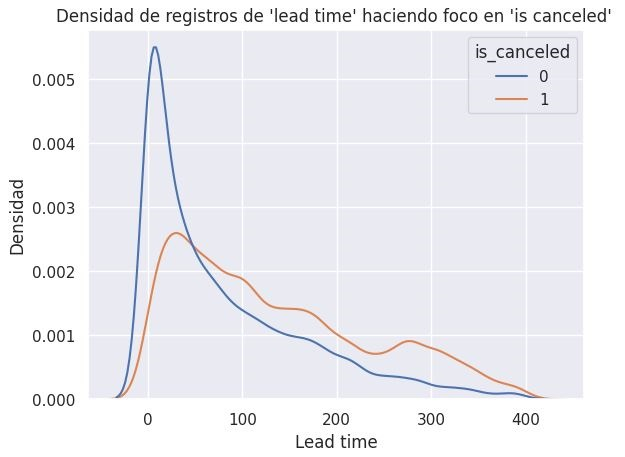
\includegraphics[scale=0.2]{lead_time}



\end{document}
